\documentclass{beamer}

\usetheme[iohk]{welltyped}
\usepackage{graphicx}
\usepackage{soul}
\graphicspath{ {../includes/} }

\begin{document}

\title{Building a Distributed System with Real-time Constraints}
\subtitle{Using concurrent Functional Programming tools}
\author{Armando Santos}
\date{\today}
\maketitle

\AtBeginSection[]{
  \begin{frame}
  \vfill
  \centering
  \begin{beamercolorbox}[sep=8pt,center,shadow=true,rounded=true]{title}
    \usebeamerfont{title}\insertsectionhead\par%
  \end{beamercolorbox}
  \vfill
  \end{frame}
}

\section{Introduction}
\subsection*{Networking Team}
\begin{frame}{Networking Team}
  \begin{columns}
    \column{.33\linewidth}
    \centering
    Armando Santos \\ Well-Typed
    \column{.34\linewidth}
    \centering
    Marcin Szamotulski \\ Input Output Global
    \column{.33\linewidth}
    \centering
    Duncan Coutts \\ Well-Typed
  \end{columns}
  \vskip1cm
  \begin{columns}
    \column{.4\linewidth}
    \centering
    Neil Davies \\ PNSol
    \column{.4\linewidth}
    \centering
    Peter Thompson \\ PNSol
  \end{columns}
\end{frame}

\section{What we are doing}

\subsection*{Cardano Node}
\begin{frame}{Cardano Node}
% Please add the following required packages to your document preamble:
% \usepackage{graphicx}
\begin{table}[]
\centering
\resizebox{\columnwidth}{!}{%
\begin{tabular}{llll}
  \multicolumn{1}{c}{\alert{\textbf{Ouroboros algorithm paper}}} &
  \multicolumn{1}{c}{\alert{\textbf{Refining step}}} &
  \multicolumn{1}{c}{\alert{\textbf{Implementation}}} &
  \multicolumn{1}{c}{\alert{\textbf{Testing}}} \\ \\
\multicolumn{1}{l|}{\begin{tabular}[c]{@{}l@{}}Formal Specification\\ \\  Threat models\\ \\  Non-realistic assumptions\\ \\  Performance objectives\end{tabular}} &
  \multicolumn{1}{l|}{\begin{tabular}[c]{@{}l@{}}Real time constraints\\ \\  Concurrency\\ \\  Operation \& Performance\end{tabular}} &
  \multicolumn{1}{l|}{\begin{tabular}[c]{@{}l@{}}Architecture \& Design\\ \\  Protocols\\ \\  Scale\\ \\  Exceptions \& Corner cases\end{tabular}} &
  \begin{tabular}[c]{@{}l@{}}Properties\\ \\  Simulation\\ \\  Reliability\\ \\  CI\end{tabular}
\end{tabular}%
}
\end{table}
\end{frame}

\subsection*{Decentralised Network}
\begin{frame}{Decentralised Network }
  \begin{columns}
    \begin{column}{0.6\textwidth}
      \vskip0.2cm
      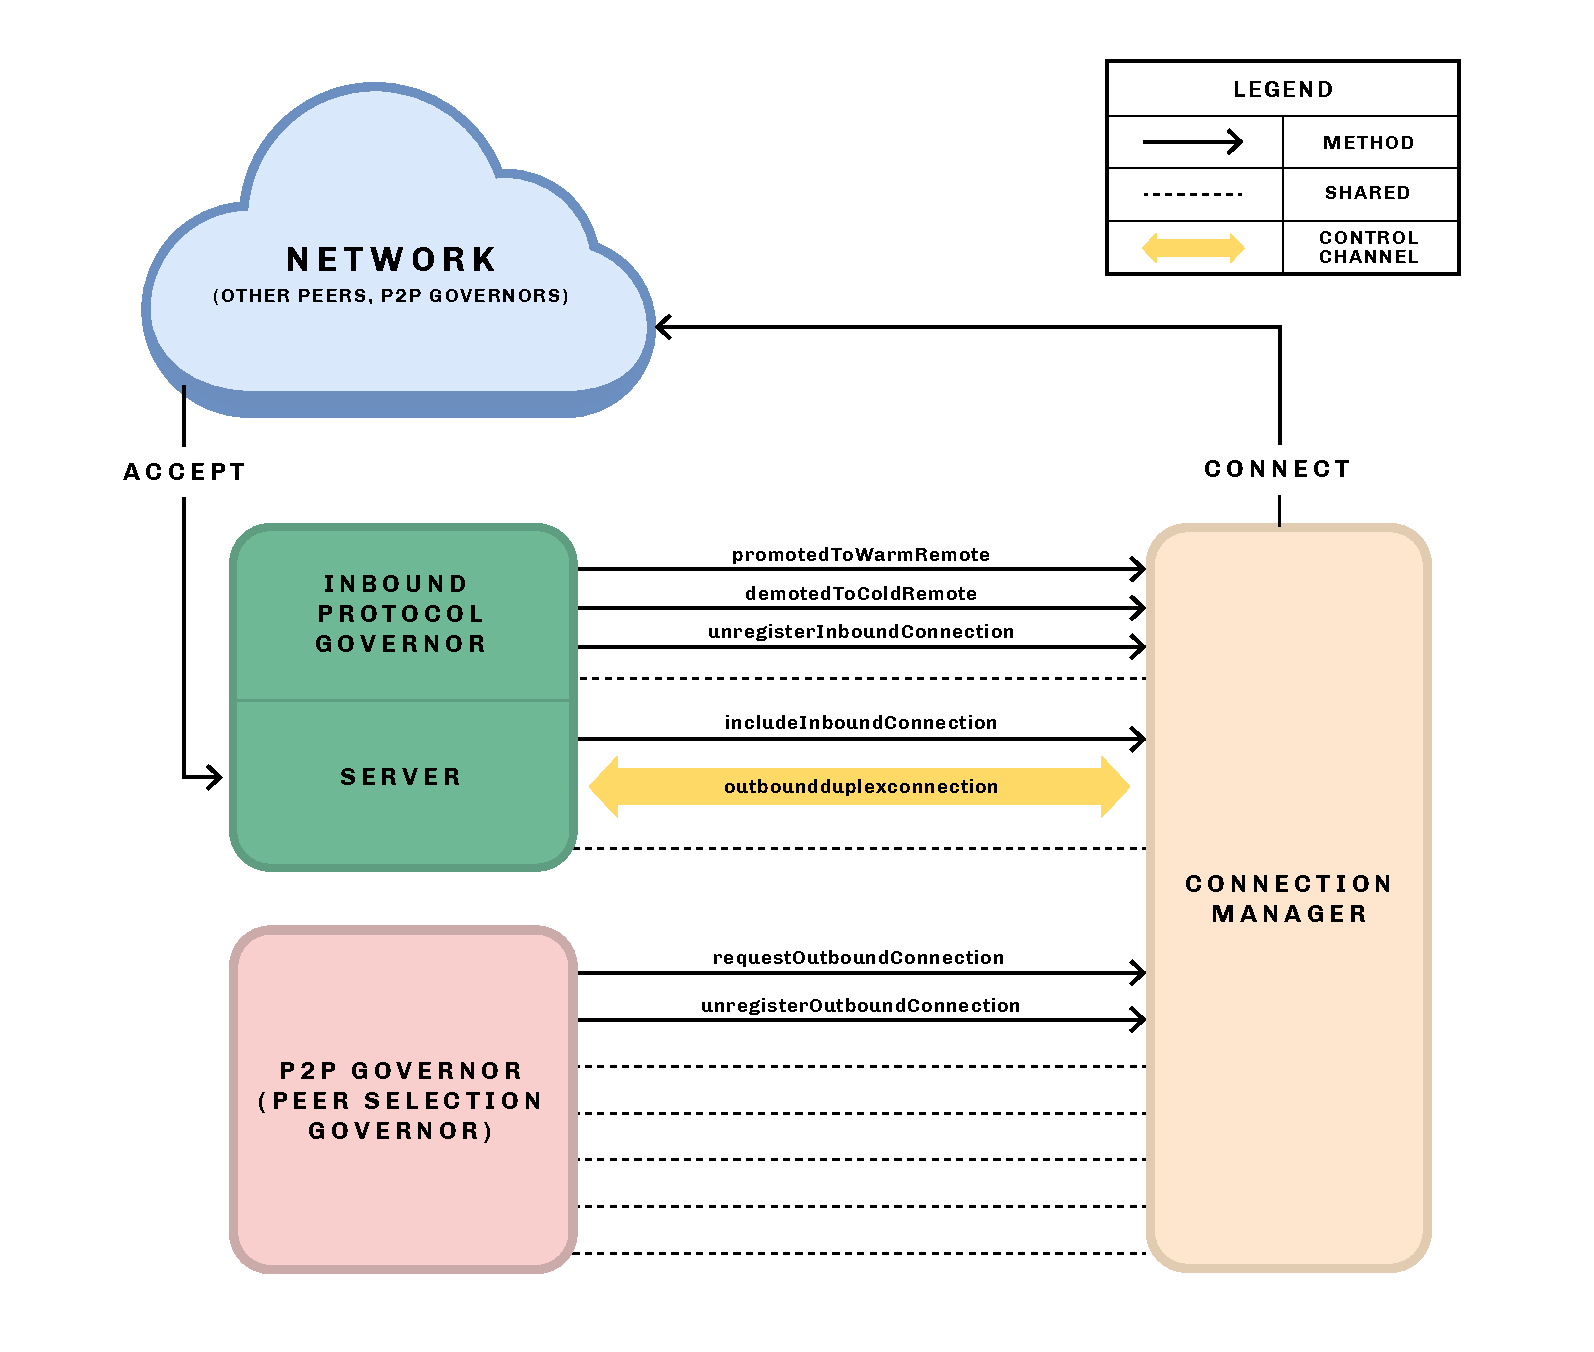
\includegraphics[height=0.9\textheight, width=\textwidth]{ConnectionManagerInteractions.pdf}
    \end{column}
    \begin{column}{0.4\textwidth}
      \footnotesize
      \begin{itemize}
        \item Highly concurrent;
        \item Reliable and Robust;
        \item Predictable;
        \item Manage resource consumption;
        \item Thousands of SPOs;
        \item Has to run 24/7.
      \end{itemize}

      \tiny
      \begin{block}{More details}
        To read more about this, check out our documentation at:
        \href{https://github.com/input-output-hk/ouroboros-network/}{https://github.com/input-output-hk/ouroboros-network/}
      \end{block}

    \end{column}
  \end{columns}
\end{frame}

\section{How we are doing it}

\subsection*{Functional Programming}

\begin{frame}{Functional Programming}
  Strongly Statically Typed Purely Functional Programming with \alert{Haskell}!

  \begin{itemize}
      \item Non-strict evaluation;
      \item \alert{Type Safeness};
      \item \alert{Referential Transparency};
      \item \alert{STM};
      \item Explicit effects;
      \item More!
  \end{itemize}

\end{frame}

\subsection*{Typed Protocols}

\begin{frame}{Typed Protocols}
  Internally developed (but open-source) library to specify end-to-end protocols at the type-level!

  \begin{itemize}
    \item Type Safe;
    \item Session Types;
    \item \alert{Deadlock free!}
    \item Pure;
    \item Powerful (pipelining out of the box).
  \end{itemize}

\end{frame}

\subsection*{QuickCheck}

\begin{frame}{QuickCheck}
  Property based testing framework for Haskell.

  \begin{itemize}
    \item \alert{Input random generation};
    \item Shrinking;
    \item \alert{Reproducibility};
    \item Coverage checks.
  \end{itemize}

\end{frame}

\subsection*{IO Simulator}
\begin{frame}{IO Simulator}
  Simulation monad that is a drop-in \alert{replacement} for IO (and other execution
  kernel primitives in Haskell)!

  Internally developed (but open source) library to perform all kinds of \alert{IO
  Simulations}, in particular:

  \begin{itemize}
    \item write \alert{network simulations}, to verify a complex networking stack;
    \item write \alert{disk IO simulations}, to verify a database implementation.
  \end{itemize}
\end{frame}

\subsubsection*{We're using IO Simulator for...}
\begin{frame}{We're using IO Simulator for...}
  \begin{columns}
    \begin{column}{0.4\textwidth}
      \begin{itemize}
        \item Early detection of critical races;
        \item Simulation of rare \alert{edge cases};
        \item Mocking and \alert{error injection};
        \item Simulate time passing;
        \item Looking for \alert{different schedules}.
      \end{itemize}
      Most importantly:
      \begin{itemize}
        \item Performing tests using \alert{same codebase} and
        \item \alert{Reproducing} complex edge-case test failures.
      \end{itemize}
    
    \end{column}
    \begin{column}{0.6\textwidth}
        %Content
      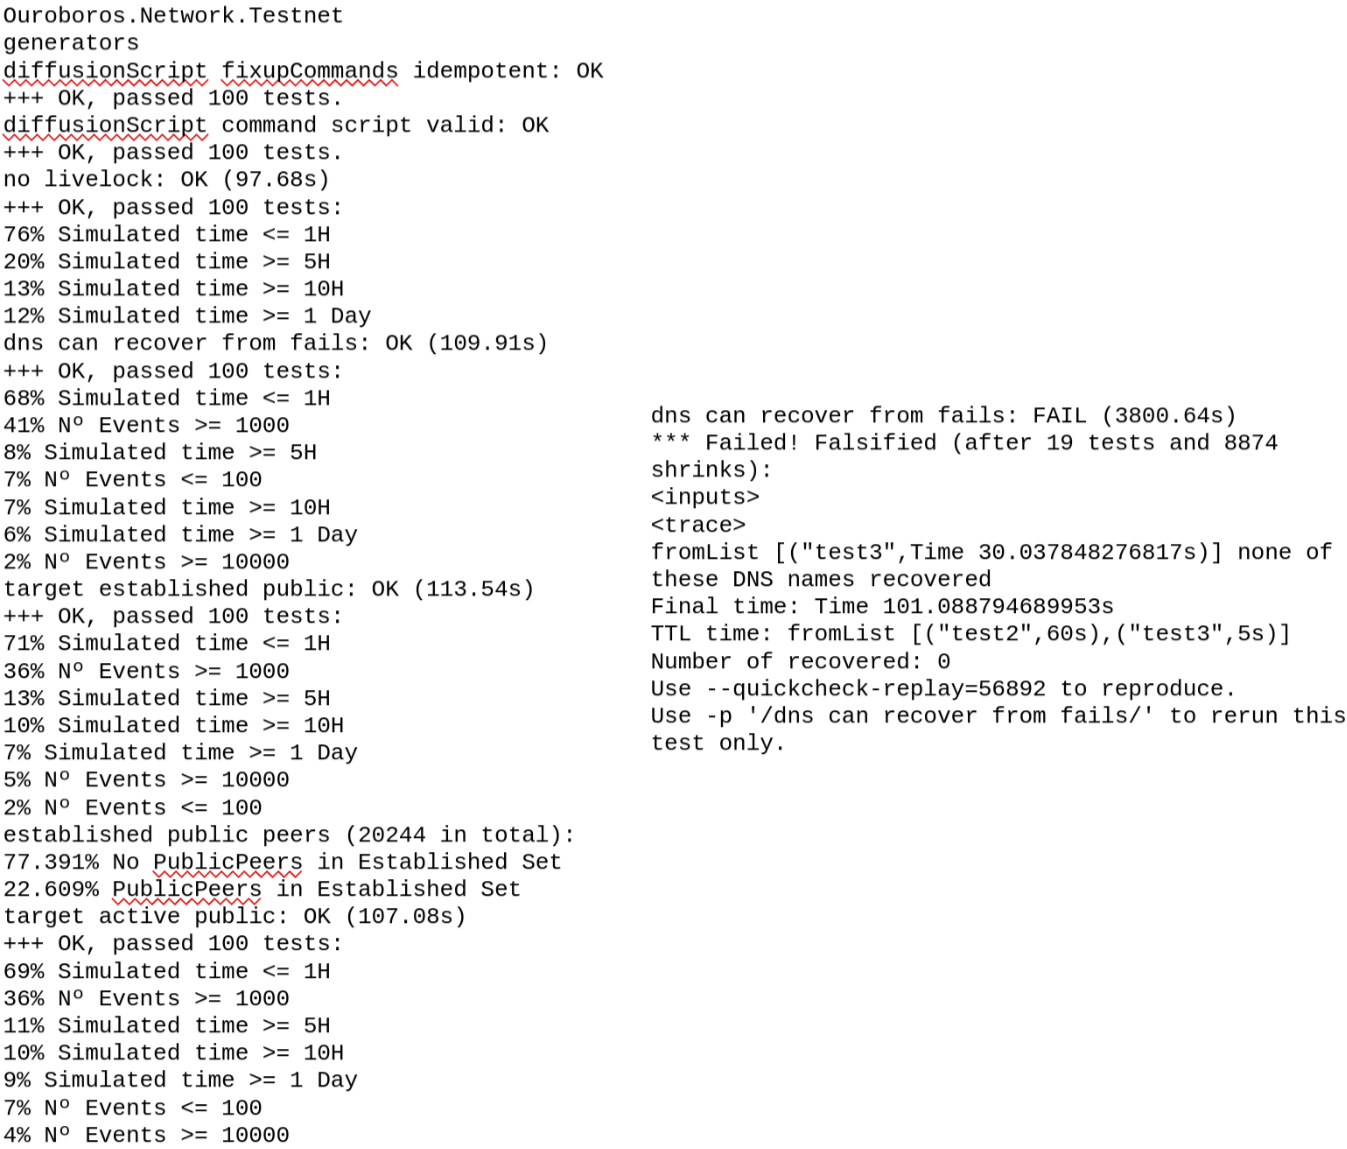
\includegraphics[scale=1.2, width=\textwidth]{code.png}
    \end{column}
  \end{columns}
\end{frame}

\section{Conclusion}

\begin{frame}{Best effort}
  \begin{itemize}
    \item Complex systems spans performance characteristics we can not control;
    \item Functional Programming, namely Haskell and its concurrency tools helped us manage complexity;
    \item We do our best in searching through all state space efficiently;
    \item Well-founded confidence;
    \item Progress is achievable.
  \end{itemize}
\end{frame}

\begin{frame}{Far from perfect}

  We have had quite a few issues, and we still do!

  \begin{itemize}
    \item \alert{378 closed issues} related with networking;
    \item \alert{276 open ones} (minor, good-to-have issues);
    \item \alert{10\%} of the issues are related with simulation environment;
    \item About a handful of them were due to misplaced logging events.
  \end{itemize}

  Our CI test suite runs on average between $1$ and $5$ hours of simulated time per test per input per PR per OS. Which means:

  \begin{itemize}
    \item Assuming around 100 tests in our test suite and
    \item each test generates 100 random inputs;
    \item Assuming 3 PRs per week;
    \item Testing on Windows, OSX and Linux;
    \item Results on around 225 000 hours of simulated time per week!
  \end{itemize}

\end{frame}

\begin{frame}{Some examples of bugs found}

  Discovering rare events in the real world:

  \begin{itemize}
    \item
      \href{https://github.com/input-output-hk/ouroboros-network/pull/3640/commits/f21334b7630c939a1ef35e452d10956cbf39e3fd}{Different
      scheduling found a edge case where state was being blindly overwritten}
    \vskip0.4cm
    \item
      \href{https://github.com/input-output-hk/ouroboros-network/issues/3572}{Asynchronous
      exceptions on a blocking \texttt{finally} block}
    \vskip0.4cm
    \item
      \href{https://github.com/input-output-hk/ouroboros-network/issues/3553}{Timeouts not
      being enforced withing reasonable bounds}
    \vskip0.4cm
    \item
      \href{https://github.com/input-output-hk/ouroboros-network/issues/3344}{Pruning
      connections misbehavior in the presence of a TCP Simultaneous Open}
  \end{itemize}

\end{frame}

\begin{frame}
  \centering
  \usebeamerfont{title}
  Thank you!
\end{frame}


\end{document}

